\documentclass[a4paper, 11pt, twoside, openany, onecolumn, final]{memoir}

\usepackage{style}

\title{\tb{Inteligencia artificial: Práctica $8$}}
\author{Álvaro García Tenorio \thanks{\texttt{\url{alvgar14@ucm.es}}}\and Miguel Pascual Domínguez\thanks{\texttt{\url{miguepas@ucm.es}}}}
\date{\today}

\begin{document}
	\maketitle
	\tableofcontents
	\chapter{Agrupamiento}
	\section{Descripción del conjunto}
	Para este experimento hemos seleccionado un conjunto de datos llamado ausencias de trabajo. Los datos pertenecen a un estudio académico realizado por la universidad Nove de Julho de Brasil, por dos estudiantes y un profesor, durante tres años desde 2007 hasta 2010 en una empresa brasileña.
	Los datos, los hemos obtenido de la siguiente pagina, \url{http://archive.ics.uci.edu/ml/datasets/Absenteeism+at+work}.
	
	Expliquemos ahora los atributos/variables de este conjunto de datos:
	
	\begin{enumerate}
\item  ID (Identificador): variable formada por un conjunto de números del 1 al 36 que consisten en 36 identificadores de 36 personas distintas.
\item Motivo de la ausencia: catalogado en 28 números que cada uno corresponde con un motivo de incidencia, los 21 primeros se tratan de las primeras 21 enfermedades del código internacional de enfermedades (ICD) y los 7 ultimos, corresponden con 7 motivos no incluidos en el ICD, que son el acompañamiento de otro paciente (22), una consulta médica (23), donación de sangre (24), análisis médico (25), ausencia injustificada (26), fisioterapia (27) y dentista (28).
\item Mes de ausencia: número real que corresponde con el mes de la ausencia del 1 al 12.
\item Día laboral de la semana: lunes (2), martes (3), miércoles (4), jueves (5) y viernes (6). 
\item Estación del año: verano (1), otoño (2), invierno (3) y primavera (4).
\item Gasto de transporte: número real.
\item Distancia desde casa hasta la oficina (km): número real.
\item Tiempo de trabajo: número entero.
\item Edad: número entero
\item Media de carga de trabajo: número real.
\item Porcentaje de cumplimento de trabajos: número real entre 0.0 y 100.0.
\item Incidencia disciplinaria: Si (1) y No (0).
\item Educación: número real, catalogado de la siguiente manera; bachillerato (1), graduado (2), posgraduado (3) y master y docotorado (4).
\item Número de hijos: número real.
\item Bebedor social: Si (1) y No (0).
\item Fumador social: Si (1) y No (0).
\item Número de mascotas: número real.
\item Peso: número real.
\item Altura: número real.
\item Índice de masa corporal: número real.
\item Tiempo de ausencia en horas: número real.
\end{enumerate}
	\section{Parametrización del algoritmo de agrupamiento}
	Veamos ahora como preparamos los datos y las variables para aplicar el algoritmo de agrupamiento jerárquico.
	
	Empecemos primero observando si tiene sentido o no estandarizar o normalizar o no hacerlas nada a las variables. Dado que algunas de ellas a pesar de que son números, realmente se les deberían considerar variables categóricas, por ejemplo el ID, el motivo de la ausencia, el día laboral, la estación del año, la incidencia disciplinaria, y el bebedor y fumador social; y por tanto al tener que considerarlas así, no tendría ningún sentido realizarles ajuste numérico.
	
	Fijemonos ahora en el resto de las variables,   AQUI FALTA DECIR PORQUE LAS OTRAS VARIABLES NO LAS ESTANDARIZAMOS NI NORMALIZAMOS PERO NO SE ARGUMENTAR PORQUE (PORQUE LA RAZON QUE SE ME OCURRE ES PURA "PEREZA").
	
	Decidamos ahora el número de clusters que queremos para nuestro agrupamiento, para ello tenemos que observar que dependiendo de que variable tomamos como principal, se necesitará un número o otro, por ejemplo si cogemos como variable, el día laboral, lo interesante sería tomar como número de clusters igual a 5, para observar como el algoritmo te agrupa por cada día laboral o por ejemplo por el motivo de la ausencia, o la estación del año, etc.
	Por todo esto, hemos decidido optar por 
	\section{Resultados}
	\section{Conclusiones y respuestas}
	\chapter{Clasificación}
		\section{Descripción del conjunto}
		Para este tipo de problema, lo interesante es coger un conjunto/database que tenga pocos atributos y muchas instancias, por ello el conjunto que hemos seleccionado es un dataset sobre una evaluación de coches, hemos obtenido los datos de la siguiente página \url{http://archive.ics.uci.edu/ml/datasets/Car+Evaluation}. Los archivos descargados no venían en formato .arff, por tanto hemos tenido que añadir parte del codigo de definición de atributos y de la relación, pero los datos no han sido modificados.
		
		Expliquemos ahora los atributos/variables, todos ellos categóricos, ninguno numérico; de este conjunto de datos:
	
	\begin{enumerate}
\item Compra: Precio de compra; muy alto (vhigh), alto (high), medio (med) y bajo (low).
\item Mantenimiento: Precio de mantenimiento; muy alto (vhigh), alto (high), medio (med) y bajo (low).
\item Puertas: Número de puertas clasificado en 4 categorías; 2, 3, 4 y 5 o más.
\item Personas: Número de personas clasificado en 3 categorías; 2, 4 y más.
\item Maletero: Capacidad del maletero; pequeña, media y grande.
\item Seguridad: baja, media y alta. 
\item Tipo de coche según aceptabilidad: inaceptable (unacc), aceptable (acc), bueno (good) y muy bueno (vgood). 
\end{enumerate}
		
		Una vez comentado los atributos, expliquemos el problema. 

Tal y como son los datos, hemos decidido que para aprovechar el potencial de los mismos, lo más lógico es plantear el problema de clasificar la aceptabilidad de los coches en función de los otros 6 atributos, para así poder observar cuales coches son inaceptables y asi no venderlos o comprarlos; ya que así podemos observar más adelante el poder del algunos atributos como la seguridad y el número de personas que ya clasifican una cantidad considerable de los coches.

Mostramos aquí el histograma de la variable tipo de coche según aceptabilidad. 
	\begin{figure}
  		\centering
   		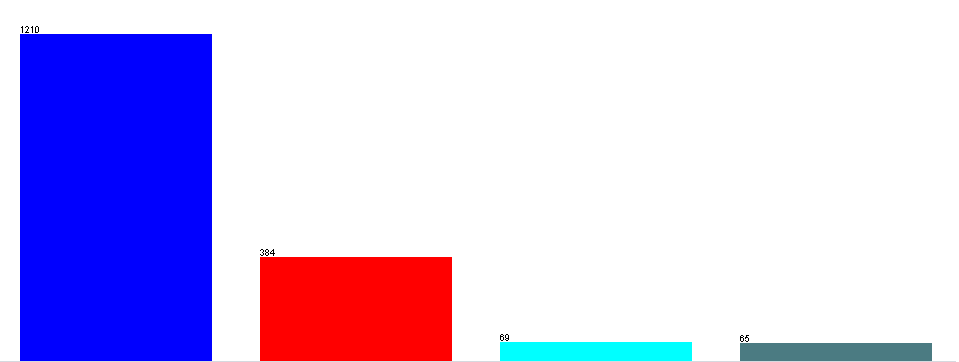
\includegraphics[width=1\textwidth]{Imagenes/HistogramaVarSalidaClasif}
  		\caption{Histograma de la variable tipo de coche según aceptabilidad}
  		\label{HistoVarSalidaClasi}
	\end{figure}
	\section{Parametrización del J48}
		Dado que todas nuestras variables son categóricas no se les puede normalizar (englobar los valores entre $0$ y $1$) ni estandarizar (modificar los datos para que tengan media $0$ y varianza $1$). 
		Primero se realizará una ejecución del algoritmo sin validación ni entrenamiento, después se realizará otra ejecución en validación y entrenamiento al $66\%$.
		
		En la primera ejecución se han mantenido los parámetros del algoritmo predeterminado por Weka y en la segunda ejecución al realizar un entrenamiento y una validación al $66\%$, vimos que el árbol resultante era muy parecido al original sin entrenamiento ni validación, por tanto decidimos añadir una nueva peculiaridad a esta segunda ejecución y era que de manera forzada siempre se realizaran particiones binarias en el árbol, es decir que formara un árbol binario.
	\section{Resultados}
	Mostremos primero los resultados de la primera ejecución, primero mostramos el sumario de weka en la Figura \ref{SumarioPrimeraEjecucion}, en el que esta incluido los valores del recall, precisión los errores y la matriz de confusión; y después el árbol en la Figura \ref{ArbolPrimeraEjecucion}.
	\begin{figure}
  		\centering
   		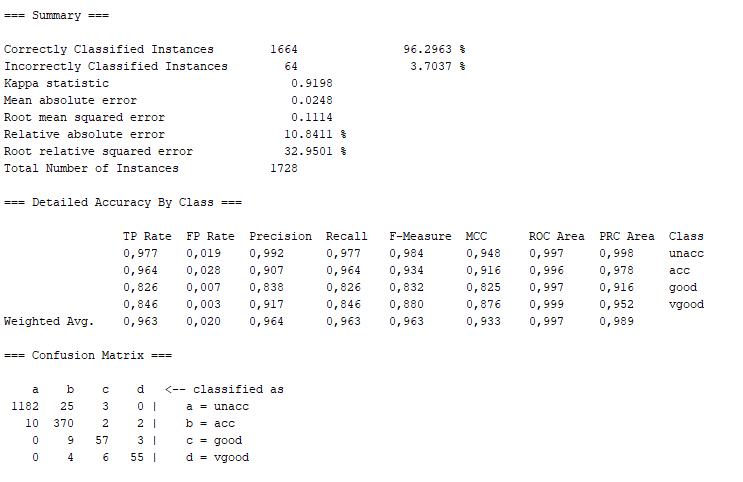
\includegraphics{Imagenes/SummarySinEntreNiVal}
  		\caption{Sumario Primera Ejecución}
  		\label{SumarioPrimeraEjecucion}
	\end{figure}	
	
	\begin{figure}
  		\centering
   		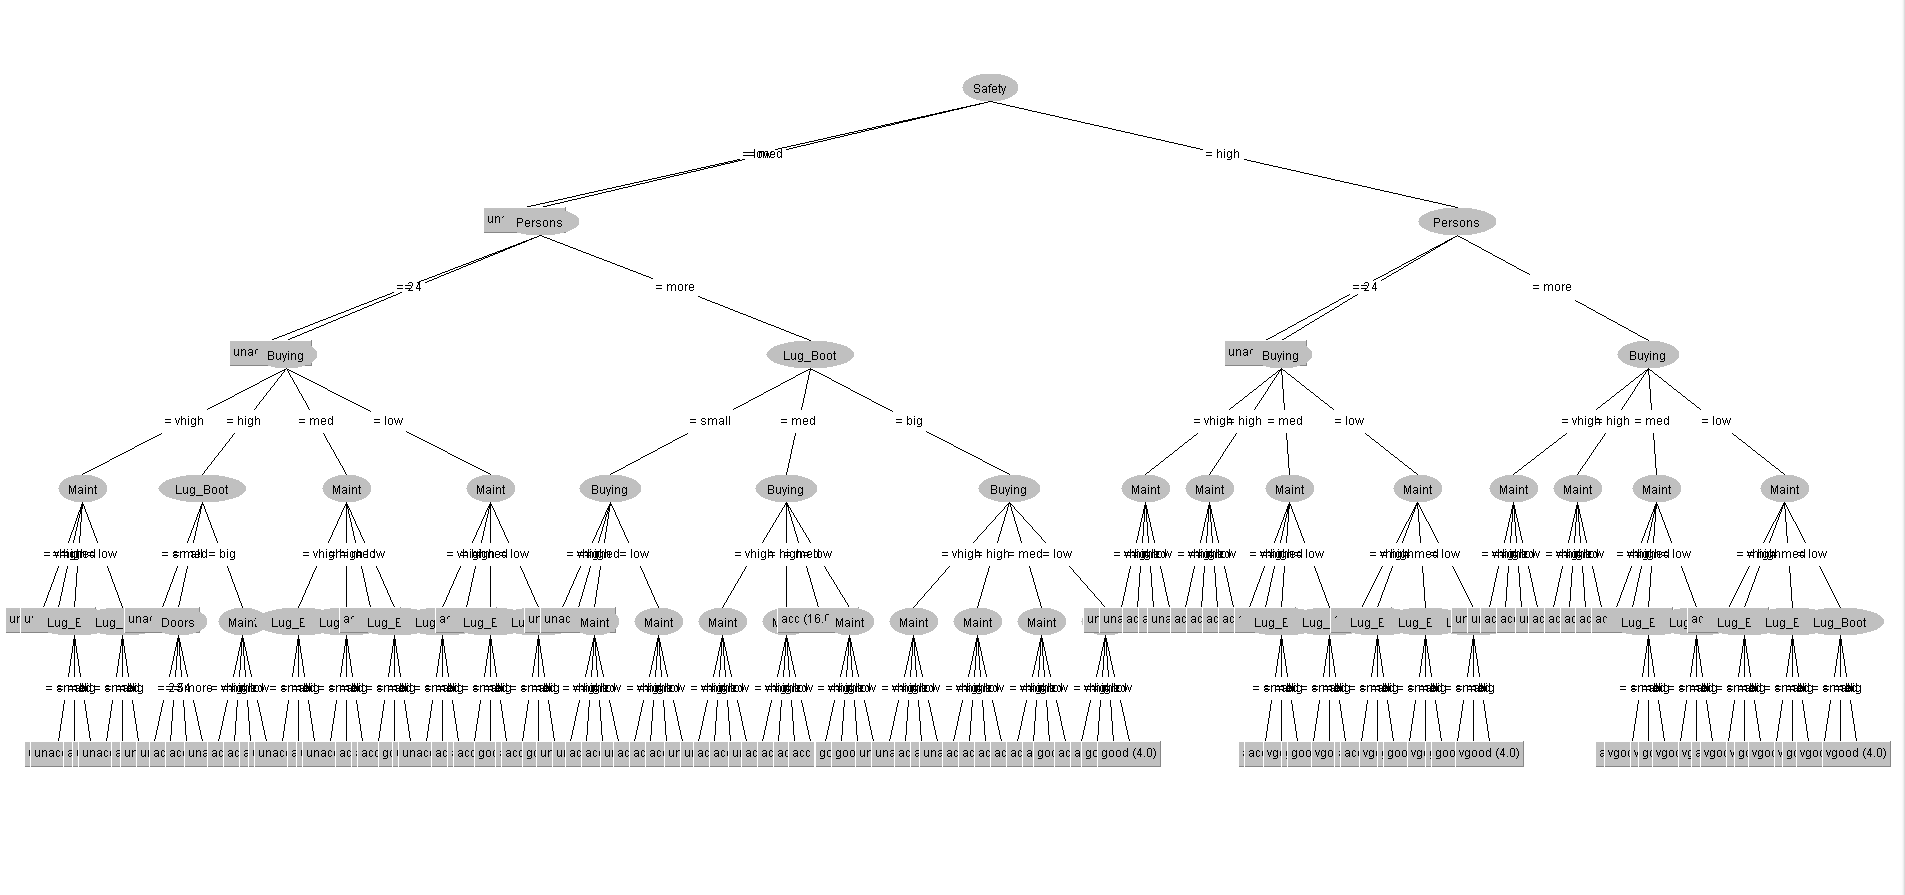
\includegraphics[width=1\textwidth]{Imagenes/ArbolSinEntreNiVal}
  		\caption{Árbol Primera Ejecución}
  		\label{ArbolPrimeraEjecucion}
	\end{figure}
	
	Mostraremos ahora los resultados de la segunda ejecución, primero mostramos el sumario de weka en la Figura \ref{SumarioSegundaEjecucion}, en el que esta incluido los valores del recall, precisión los errores y la matriz de confusión; y después el árbol en la Figura \ref{ArbolSegundaEjecucion}.
	\begin{figure}
  		\centering
   		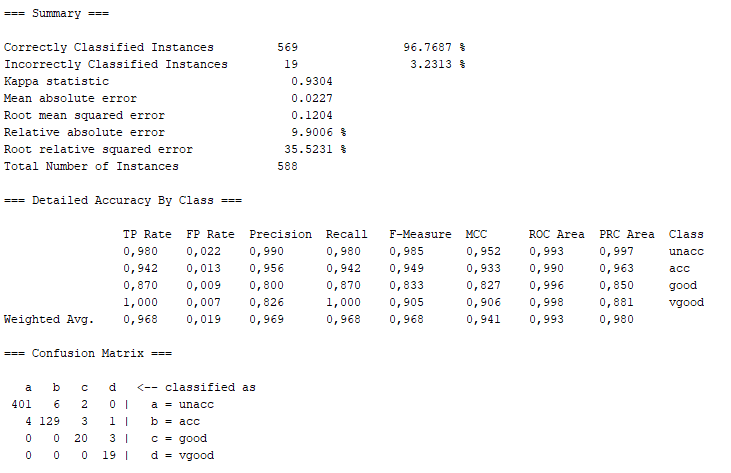
\includegraphics{Imagenes/SummaryConEntreYValYBinarySplit}
  		\caption{Sumario Primera Ejecución}
  		\label{SumarioSegundaEjecucion}
	\end{figure}	
	
	\begin{figure}
  		\centering
   		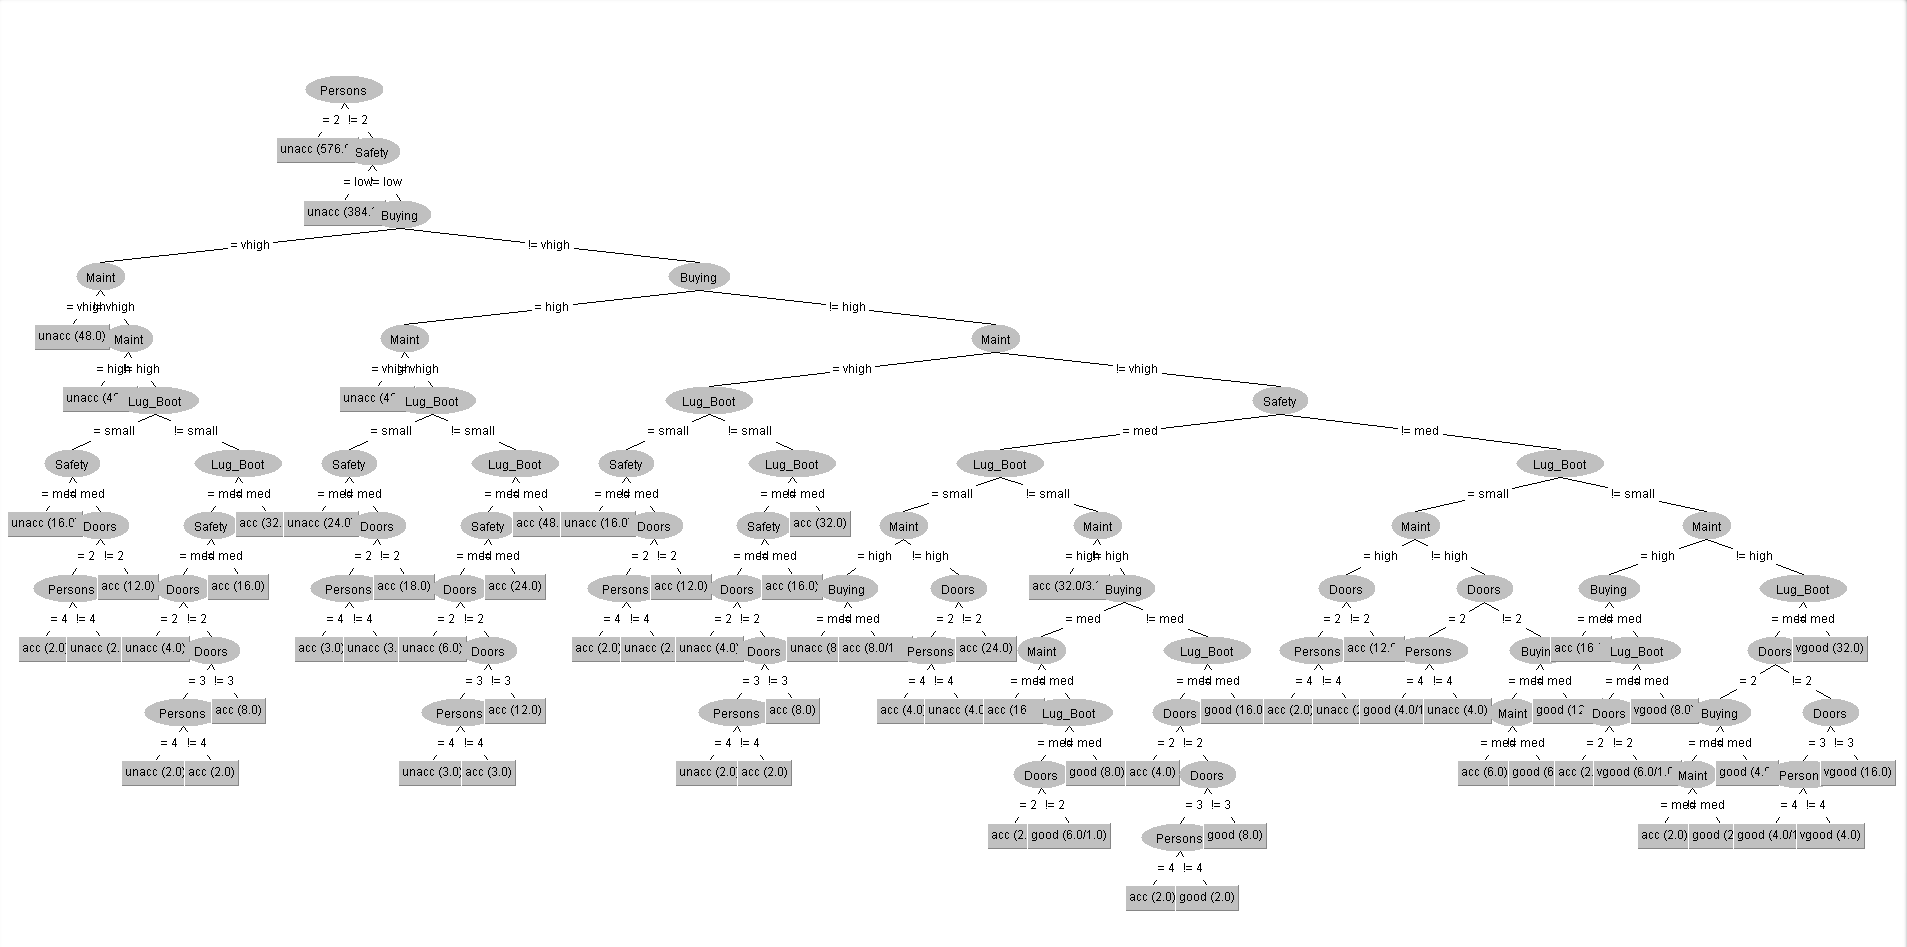
\includegraphics[width=1\textwidth]{Imagenes/ArbolConEntreYValYBinarySplit}
  		\caption{Árbol Primera Ejecución}
  		\label{ArbolSegundaEjecucion}
	\end{figure}
	
	Comentemos ahora los resultados obtenidos en ambas ejecuciones:
	
	Como se puede observar en la primera ejecución se produce un árbol más o menos claro, en el que casi todos los nodos tienen $3$ o $4$ hijos, también se observa que el algoritmo le cuesta diferenciar entre los tipos de coches que son aceptables, buenos o muy buenos; tal y como se ve en la matriz de confusión, también se observa que el porcentaje de instancias mal clasificadas es realmente bajo pues es menor de un $5\%$, lo cual es un porcentaje realmente bueno.
	
	En la segunda ejecución, decidimos forzar a al árbol para que fuera binario, lo que provoca que se cree un  árbol con mayor profundidad y menos homogéneo que el anterior, pero en cambio al realizar una parte de entrenamiento y validación, el porcentaje de fallos en la clasificación es incluso menor, en unas pocas décimas que en la primera ejecución, y además se observa en la matriz de confusión, ahora la confusión que tenía con los coches buenos y muy buenos ha dejado de tenerla. 
	
	En cambio, cabe destacar que a pesar de que la segunda ejecución presenta menos equivocación, la precisión que posee en los coches buenos, es menor que en la primera ejecución, a pesar de que la segunda tiene una precisión global mayor que en la primera ejecución, además de que la segunda parametrización posee una mayor sensibilidad a la hora de concretar en los tipos de coches según aceptabilidad.
	
	\section{Conclusiones y respuestas}
	Por la claridad, y la manera de filtrar que realiza, consideramos que es mejor árbol el de la primera ejecución a pesar de que se confunde en algunas instancias, pero para interpretar el problema, consideramos que se obtiene una interpretación mejor que con la segunda ejecución. Las principales diferencias se encuentran en las ramas iniciales, al ser el primero un árbol con una raíz con mas de dos hijos, hay más claridad y orden en el árbol. 
	
	En cambio en términos de validación consideramos que el segundo árbol es más exacto y con mejores estadísticas que la primera ejecución.
	
	Interpretemos ahora el primer árbol para responder las preguntas en función del contexto del problema.
	
	La raíz del árbol evalúa el atributo de seguridad de un coche, la cual es una de las preguntas mas importantes a la hora de valorar si un coche es aceptable o no, pues un coche seguro es a nuestro punto de vista uno de los vehículos mas peligrosos. Por ello como se puede observar, los coches que mejor ha clasificado y acertado han sido los coches inaceptables (unacc).
	
	Como hemos comentado la seguridad ha sido una de las variables mas relevantes en el problema, además de que es el nodo que más poder discriminante tiene, y a pesar de esto en la segunda ejecución no se ha tomado la seguridad en la raíz sino que se ha tomado el número de personas, a pesar de que están en el mismo nivel, lo cual esto se puede deber al algoritmo de selección interno de weka y que al exigirle la distinción binaria, hace que el número de personas tenga un mayor poder discriminante.   
	
	En efecto, se puede observar que hay dos variables que se confunden sobretodo entre si que son las dos relacionadas con el precio, buying y maint; a lo largo de todo el árbol pues normalmente, son las clases que menos discriminan y se seleccionan las últimas,y que además están organizados con los mismos valores, muy alto (vhigh), alto (high), medio (med) y bajo (low). Tiene cierto sentido que se confundan pues normalmente un coche que cueste mucho dinero, también va a tener un mantenimiento de coste alto. 
	
	Además a nuestro punto de vista, estas dos clases junto con la del tamaño del maletero, son las clases que menos información aportan, pues al final son las que clasifican entre los buenos coches, que si enfocamos este problema simplemente para descartar los coches peligrosos/inaceptables, dichas clases no nos darían información relevante.
	
	\chapter{Regresión}
		\section{Descripción del conjunto}
	\section{Parametrización del perceptrón multicapa}
	\section{Parametrización del K-NN}
	\section{Resultados}
	\section{Conclusiones}
\end{document}